%%%%%%%%%%%%%%%%%%%%%%%%%%%%%%%%%%%%%%%%%%%%%%%%%%%%%%%%%%%%%%%%%%%%%%%%%%%%%%%%
%2345678901234567890123456789012345678901234567890123456789012345678901234567890
%        1         2         3         4         5         6         7         8

\documentclass[letterpaper, 10pt, conference]{ieeeconf}  % Comment this line out if you need a4paper

%\documentclass[a4paper, 10pt, conference]{ieeeconf}      % Use this line for a4 paper

\IEEEoverridecommandlockouts                              % This command is only needed if 
                                                          % you want to use the \thanks command

\overrideIEEEmargins                                      % Needed to meet printer requirements.

% See the \addtolength command later in the file to balance the column lengths
% on the last page of the document

% The following packages can be found on http:\\www.ctan.org
\usepackage{graphics} % for pdf, bitmapped graphics files
%\usepackage{epsfig} % for postscript graphics files
%\usepackage{mathptmx} % assumes new font selection scheme installed
%\usepackage{times} % assumes new font selection scheme installed
\usepackage{amsmath} % assumes amsmath package installed
\usepackage{amssymb}  % assumes amsmath package installed
\usepackage[noadjust]{cite}
\usepackage{lipsum}
\usepackage{float}
\usepackage{multicol}
\usepackage{siunitx}
\usepackage{pdfpages}
\usepackage{subfigure}

\title{\LARGE \bf
Audio-Sheet Music Alignment using Soft Bootleg Score Synthesis
}


\author{Teerapat Jenrungrot \\
        Department of Engineering \\
        Harvey Mudd College, Claremont, CA USA \\
        {\tt\small mjenrungrot@hmc.edu}%
}


\begin{document}

% - Fore material - title, name, date, abstract (5 pts)
% - Introduction - clear problem statement, provides appropriate context (5 pts)
% - System design - clear explanation of proposed approach block diagram, provide clear rationale for design, demonstrates thoughtful design process with iterative development (20 pts)
% - Results - implements proposed system, presents empirical results on a non-trivial data set, uses appropriate evaluation metrics (30 pts)
% - Discussion - thougtful discussion and interpretation of results, includes additional followup experiments or analyses to provide deeper insight and intuition (20 pts)


\maketitle
\thispagestyle{empty}
\pagestyle{empty}


%%%%%%%%%%%%%%%%%%%%%%%%%%%%%%%%%%%%%%%%%%%%%%%%%%%%%%%%%%%%%%%%%%%%%%%%%%%%%%%%
\begin{abstract}

Audio-sheet music alignment is the task of finding the correspondences between a time instant of an audio signal and its corresponding sheet music images. Our method converts audio data to its log-frequency spectrogram and later to a crude representation of the score that only contains rectangular floating notehead blobs, a process we call bootleg score synthesis. We next align the bootleg representation with the sheet music images using a simple variant of dynamic time warping. On the synthetic MSMD dataset, we compare our proposed system with other baseline systems including the state-of-the-art system based on deep reinforcement learning. Our method achieves 80\% accuracy at an error tolerance of 400 pixels, which is about half of a single line in sheet music.

\end{abstract}

%%%%%%%%%%%%%%%%%%%%%%%%%%%%%%%%%%%%%%%%%%%%%%%%%%%%%%%%%%%%%%%%%%%%%%%%%%%%%%%%
\section{INTRODUCTION}
This paper addresses the problem of score following in sheet music images. The task of an automatic score following system is to create a temporal alignment between time instances of a musical performance and its corresponding known symbolic representation, the score. The objective is to minimize an error between the predicted locations and actual pixel locations on the sheet music. Score following problem is a basis of many subsequent applications such as page turning \cite{page_turning}, automatic accompaniment \cite{accompaniment1, accompaniment2}, and the synchronization of visualization of the live music during concerts \cite{live1, live2}.

Several previous works have studied the problem of audio-sheet music alignment. There are two main approaches to this problem. The first approach is based on an existing optimal music recognition (OMR) software to convert sheet music into a MIDI representation and then to compare the MIDI and audio based on chroma representation \cite{omr_based1, omr_based2}. The second more recent approach is based on convolutional neural networks (CNNs). This approach attempts to learn a multimodal network that can learn the joint representation of sheet music and audio \cite{dorfer2, dorfer3}. Another recent work \cite{dorfer} attempts to formulate the audio-sheet music alignment problem as a deep reinforcement learning game where the agent has to navigate through the score by adopting its reading speed in reaction to the currently playing performance. Even though this work \cite{dorfer} achieved a state-of-the-art performance on a synthetic dataset \cite{msmd}, the method requires significant amount of training in a simulated environment that the agents have to interact with. Such issue makes the method very challenging to train an agent that generalizes well to unseen pieces and audio conditions, even if there exists many techniques such as weight-decay, dropout, or batch-normalization to make an algorithm generalize better by using regularization.

The task of score following is also closely related to the problem of audio synchronization. In the audio synchronization problem, the objective is to find a temporal alignment between two different audio recordings of the same musical piece playing at different speed. The main technique used to solve this alignment problem is a dynamic programming algorithm named dynamic time warping (DTW) \cite{dtw1, dtw2}. Many works have proposed an extension to DTW algorithm to work in online fashion, estimate the alignment at multiple granularities, handle jumps or partial alignment, and take advantage of multiple recordings. Though many works have been explored on audio alignment, there are not many works on multimodal alignment such as directly aligning sheet music and audio recording.

While many recent works have been particularly focusing on developing techniques based on CNNs to learn a joint representation of audio and sheet music to solve sheet music following problem, this paper proposes a simple approach for aligning between an audio performance with its corresponding symbolic representation a simple variant of DTW algorithm through a crude representation of sheet music containing only noteheads. An input audio signal is converted to its log-frequency spectrogram for generating its bootleg representation. The bootleg representation is then aligned with sheet music using the DTW algorithm. Previous works on cross-modal alignment have mainly focused either on using OMR to bridge the modality gap or indirectly learning a representation in the image domain. In contrast, our approach converts audio signal to its bootleg representation and uses DTW algorithm to compute alignment in image domain.

The paper is organized as follows: Section II describes the proposed system. Section III explains the experimental setup. Section IV presents the results, and Section V concludes the work with possible future directions.

\section{SYSTEM DESIGN}
There are two inputs to our system: an audio performance and its corresponding sheet music. Similar to other recent works on score following \cite{dorfer, dorfer2, dorfer3}, we assume that the sheet music is given as a sequence of image strips, where each image strip contains a single grand staff containing an upper staff (treble clef) and a lower staff (bass clef). In this work, we primarily focus on piano music. The image strips may have different dimension and the location of the staff lines may appear at different locations. Our proposed method consists of multiple steps as depicted by Figure \ref{fig:system_overview}. 

The description of the system is organized into three subparts: (1) data preprocessing where we convert audio to its log-frequency spectrogram and detect staff line locations from sheet music strips, (2) bootleg synthesis where we generate the bootleg representation based on the log-frequency spectrogram and the detected staff line locations, and (3) DTW algorithm whose goal is to construct a temporal alignment between a sequence of sheet music strips and the bootleg representation.

\begin{figure*}
    \centering
    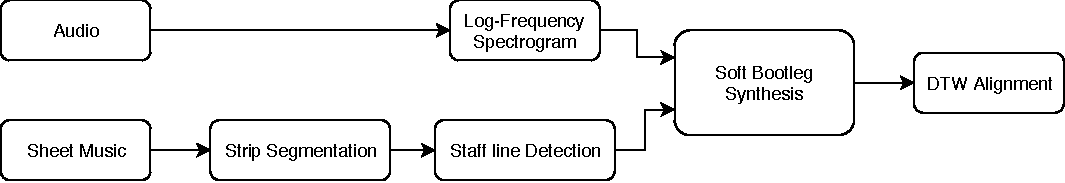
\includegraphics[width=\textwidth]{images/SystemOverview.pdf}
    \caption{System Overview. From audio signal, we compute log-frequency spectrogram. From sheet music, we segment it to a sequence of strips and perform staff line detection individually. With the log-frequency spectrogram and staff line coordinate system, we synthesize the bootleg representation and finally do the DTW alignment between the bootleg representation and sheet music strips.}
    \label{fig:system_overview}
\end{figure*}

\subsection{Data Preprocessing}
In data preprocessing step, the goal is to convert audio signal to its log-frequency spectrogram and to detect staff line locations in sheet music strips.

To compute the log-frequency spectrogram of the input audio signal, we use \texttt{madmom} library \cite{madmom} to compute the log-frequency spectrogram with a sample rate of \SI{22050}{Hz}, an FFT window size of 2048 samples, and a frame rate of 20 frames per second. In the log-frequency spectrogram, we only use the frequency in the interval between the note C1 ($f = \SI{32.70}{Hz}$) to the note C8 ($f = \SI{4186.01}{Hz}$). For the dimension of the log-frequency spectrogram, we precisely set the number of spectrogram's bins equal to 1 bin per semitone or 12 bins per octave.

The next step is to convert sheet music into a sequence of strips. Recall that a strip is a single line of sheet music. Because this paper primarily focuses on piano sheet music, a single strip consists of a single grand staff that has a upper staff (treble clef) and a lower staff (bass clef). Similar to previous works on sheet music following \cite{dorfer,dorfer2,dorfer3,msmd}, we assume that we can split sheet music into a sequence of strips perfectly. Note that each strip may have different dimension due to the format of a sheet music page.

The final step of data preprocessing is to detect staff line locations. The objective of this step is to estimate the vertical pixel location for each of the 10 lines in the grand staff for each image strip. We do this by computing the row sum of image pixels, convolving the result with comb filters of various sizes (each containing 5 regularly spaced impulses), and identifying the comb filter that yields the strongest response at two non-overlapping staff locations. This gives us the staff line coordinate system for the upper and lower staves that will be used to construct the bootleg representation.

\subsection{Bootleg Synthesis}

\begin{figure}
    \centering
    \hspace*{-2cm}
    \subfigure[Sheet music strip]{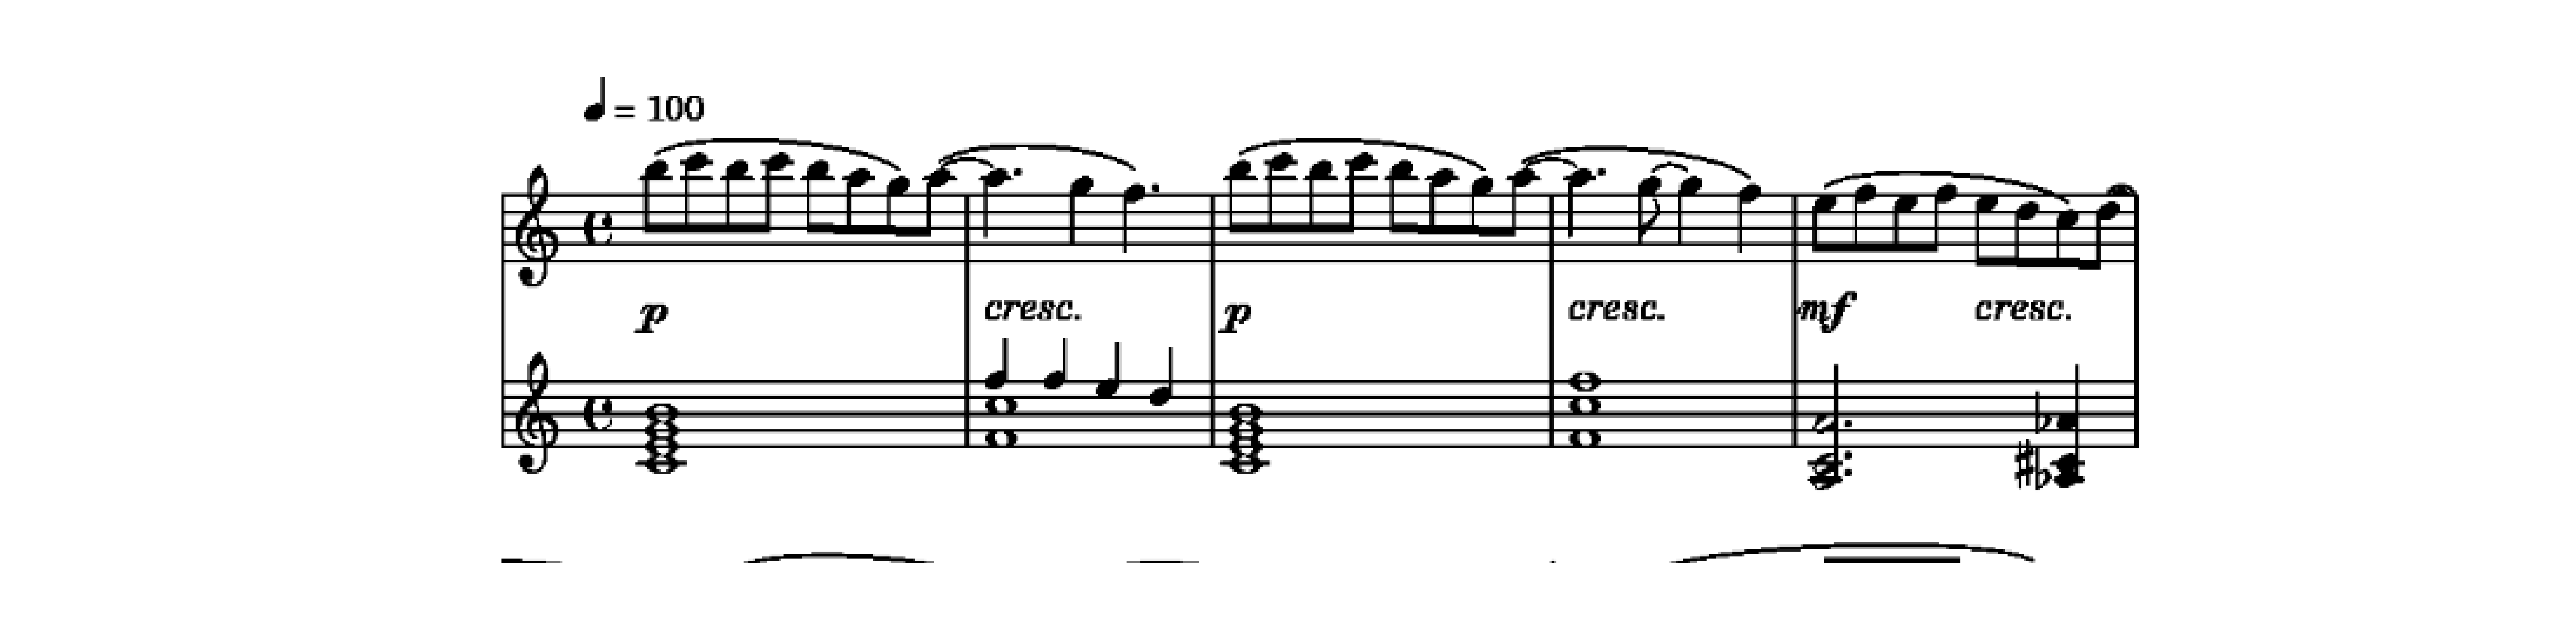
\includegraphics[scale=0.22]{images/sheetmusic.png}}
    \hspace*{-2cm}
    \subfigure[Synthesized bootleg]{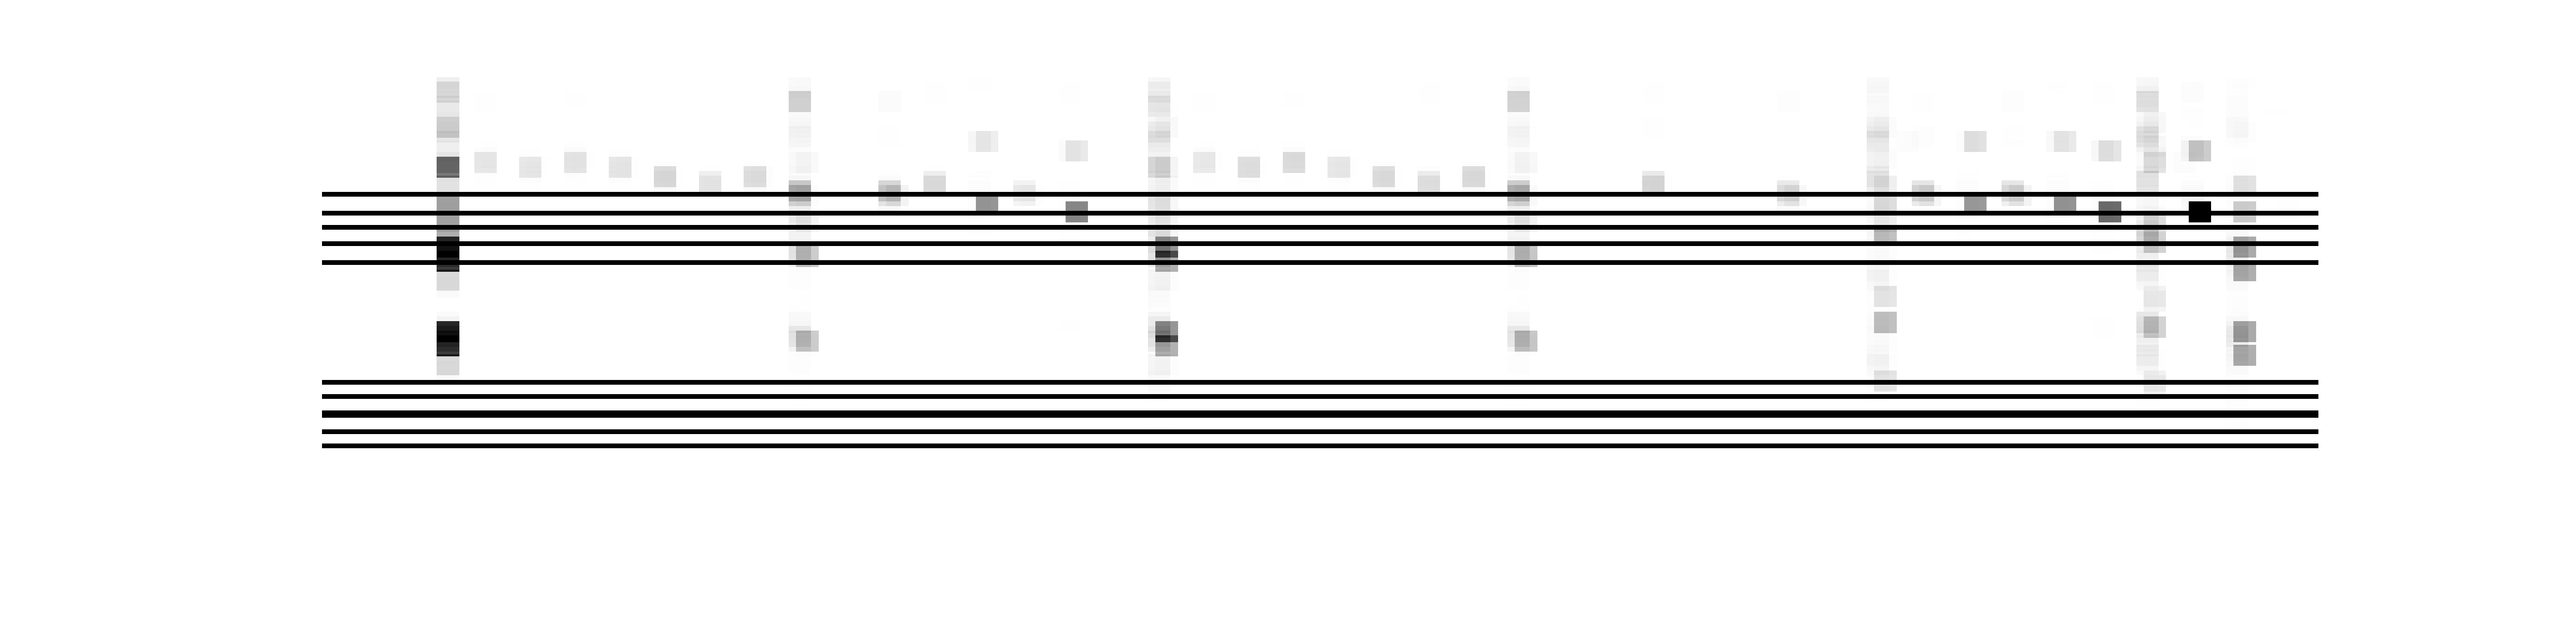
\includegraphics[scale=0.22]{images/bootleg.png}}
    \caption{Comparison between (a) sheet music strip and (b) the corresponding synthesized bootleg score. In (b), the floating notehead blobs only stay in the upper staff because both upper and lower staves have treble clefs.}
    \label{fig:bootleg}
\end{figure}

In bootleg synthesis step, the objective is to create a bootleg representation that resembles a sparse, rough estimation of sheet music containing only noteheads using a log-frequency spectrogram and staff line coordinate system. Figure \ref{fig:bootleg} visualizes a bootleg representation. 

The first step is to compute novelty function to locate sudden change in energy of an arbitrary pitch between C1 and C8 in any consecutive frame in the log-frequency spectrogram. Similar to an energy-based novelty function for onset detection in music signals \cite{onset}, the Equation \ref{eq:novelty_func} defines the novelty function for pitch $f$ at frame $n$.
\begin{equation}
    \Delta(n,f) = \begin{cases}
        S(0,f) & \text{if $n = 0$} \\
        \text{ReLU}(S(n,f) - S(n-1,f)) & \text{otherwise}
    \end{cases}
    \label{eq:novelty_func}
\end{equation}
where $S(n,f)$ is the log-frequency spectrogram at frame $n$ and pitch $f$ and $\text{ReLU}(x)$ is a half-wave rectifier defined by
\begin{equation}
    \text{ReLU}(x) = \begin{cases}
        0 & \text{if $x < 0$} \\
        x & \text{otherwise}
    \end{cases}.
    \label{eq:half_wave}
\end{equation}

The second step is to compute the note onset likelihood matrix. The note onset likelihood matrix is a matrix of the same size as the log-frequency spectrogram that provides a numerical approximation of the likelihood of observing pitch $f$ on $n$-th frame in the log-frequency spectrogram. We use Equation \ref{eq:note_likelihood} to compute the note onset likelihood at frame $n$ and pitch $f$:
\begin{equation}
    I(n,f) = \left(\frac{\Delta(n,f)}{M}\right)^2 
    \label{eq:note_likelihood}
\end{equation}
where $M = \max\limits_{n,f}\Delta(n,f)$ is the normalization factor. We squared the ratio in order to penalize lower values.

The third step is to synthesize and place noteheads. Given the staff line coordinate system from an image strip, we map the note onset likelihood into one or more floating rectangular noteheads. Note that the value of the note onset likelihood stays between 0 and 1. A note onset likelihood of 1 indicates the strongest likelihood of presence of note onset. We then create a rectangular blob with the value of note onset likelihood based on its pitch and the staff line locations. Since a value of note onset likelihood determines the value of the rectangular blob, we called this representation a `soft' bootleg. Note that there is an ambiguity when converting from a note number in the log-frequency spectrogram and its symbolic representation. For instance, a note G-sharp and A-flat both have high energy in the same frequency bin, but the symbolic representation is different. To resolve this issue, we can place a larger-than-normal rectangular notehead that overlaps both possible locations. Furthermore, notes in the middle register could appear in the right hand or left hand staves. To handle this ambiguity, we simply place two different floating noteheads at both possible locations.

The fourth step is to handle timing issues. When converting the log-frequency spectrogram into the bootleg representation, we need to specify how much time corresponds to a single pixel column. To avoid extreme warping, we select this parameter to ensure that the bootleg representation is approximately the same length as the image strips concatenated end-to-end.

Given the staff line locations, this process generates a bootleg score representation of the entire performance ($B_i$ in Figure \ref{fig:dtw}). Because each sheet image strip $i$ has a different size and a different staff line coordinate system, we generate one bootleg score $B_i$ for each image strip $i$. In other words, $B_i$ is the bootleg score representation based on the log-frequency spectrogram data projected onto the staff line coordinate system of image strip $i$. Note that all of the bootleg score representations will have the same length (i.e. number of pixel columns), but each $B_i$ will have a unique height that matches the height of image strip $A_i$.

\subsection{DTW Alignment}

\begin{figure}
    \centering
    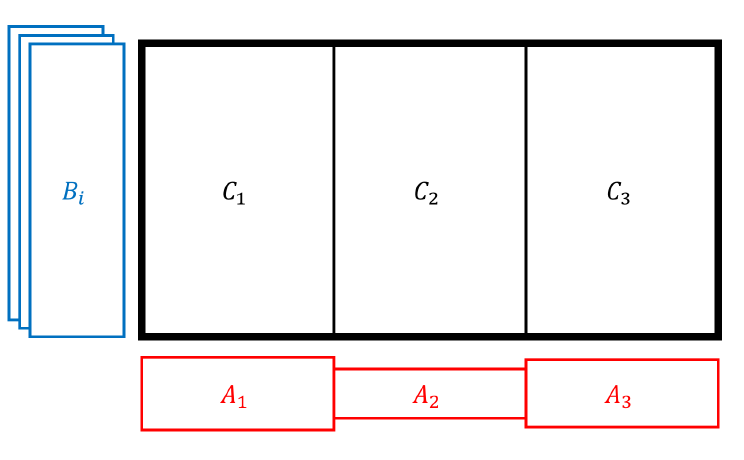
\includegraphics[scale=0.45]{images/dtw.PNG}
    \caption{Aligning generated bootleg scores with the sheet image-generated bootleg strips. Each sheet music strip $A_i$ is compared to its corresponding bootleg score $B_i$ to yield a cost matrix block $C_i$. Note that each $B_i$ is a generated bootleg score of the entire piece projected onto the staff line coordinate system of strip $A_i$.}
    \label{fig:dtw}
\end{figure}

With sheet music and the bootleg representation, we now aim to align these two visual representations using a simple DTW algorithm. Figure \ref{fig:dtw} shows a graphical illustration of this process. Suppose $A_i$ is the $i$-th sheet music strip. We construct the bootleg representation $B_i$ based on $A_i$'s staff line coordinate system and compute the cost matrix block $C_i$ by using a simple negative inner product. The $(k,\ell)$-th element of $C_i$ thus indicates the similarity between $k$-th pixel column of $b_i$ and the $\ell$-th pixel column of $A_i$. We assemble the constituent cost matrices $C_i$ into a single global cost matrix (represented as a bold black rectangle in Figure \ref{fig:dtw}), and then apply DTW with step transitions $\{(1, 1), (1, 2), (2, 1)\}$ and corresponding weights $\{2,3,3\}$. The lowest cost path through the global cost matrix is the estimated alignment between sheet music and the corresponding performance.

\section{EXPERIMENTAL SETUP}
In this section, we analyzed our system with three other baseline systems. The first baseline system is the global linear baseline system. In the global linear baseline system, we assume that the time instance of log-frequency spectrogram has a linear correspondence with the sheet music. The second baseline system is similar to our proposed system with the salience representation of audio instead of the pure log-frequency spectrogram. In this baseline system, we only replace the log-frequency spectrogram with its salience representation that sums up 8 harmonics from the fundamental frequencies. The third baseline system is the recent state-of-the-art score following using deep reinforcement learning \cite{dorfer}.

In evaluating the system's performance, we used the multimodal sheet music dataset (MSMD). The MSMD dataset contains 479 classical piano pieces from various composers. For each musical piece, the dataset provides its sheet music in PDF format, pixel locations of all noteheads and staves of the symbolic representation, the corresponding MIDI files, and the temporal alignment between the pixel locations of noteheads and time instances in the MIDI files. The dataset has also provided 4 different soundfonts for synthesizing audio. 

Since the third baseline system using deep reinforcement learning \cite{dorfer} trains the network on a subset of these 479 pieces, we decided to evaluate our system only on the same test split containing 100 pieces. This test splits contains 131 sheet music pages, \SI{29851}{~}noteheads, and \SI{29321}{~}alignment pairs. To synthesize audio, we used a software named \cite{fluidsynth} with the same parameters as indicated by the MSMD dataset. We evaluated the performance of our system together with three other baseline systems using only one soundfont.

The evaluation metrics are the error tolerance curve, the mean absolute error, $\overline{|d_x|}$, and the standard deviation of absolute error, $std(|d_x|)$. The error tolerance curve indicates the percentages of the prediction of the note onset locations are within the specified threshold. The mean absolute error and the standard deviation are the average and the standard deviation of all predictive of note onset locations.

\section{RESULTS}

\begin{figure}
    \centering
    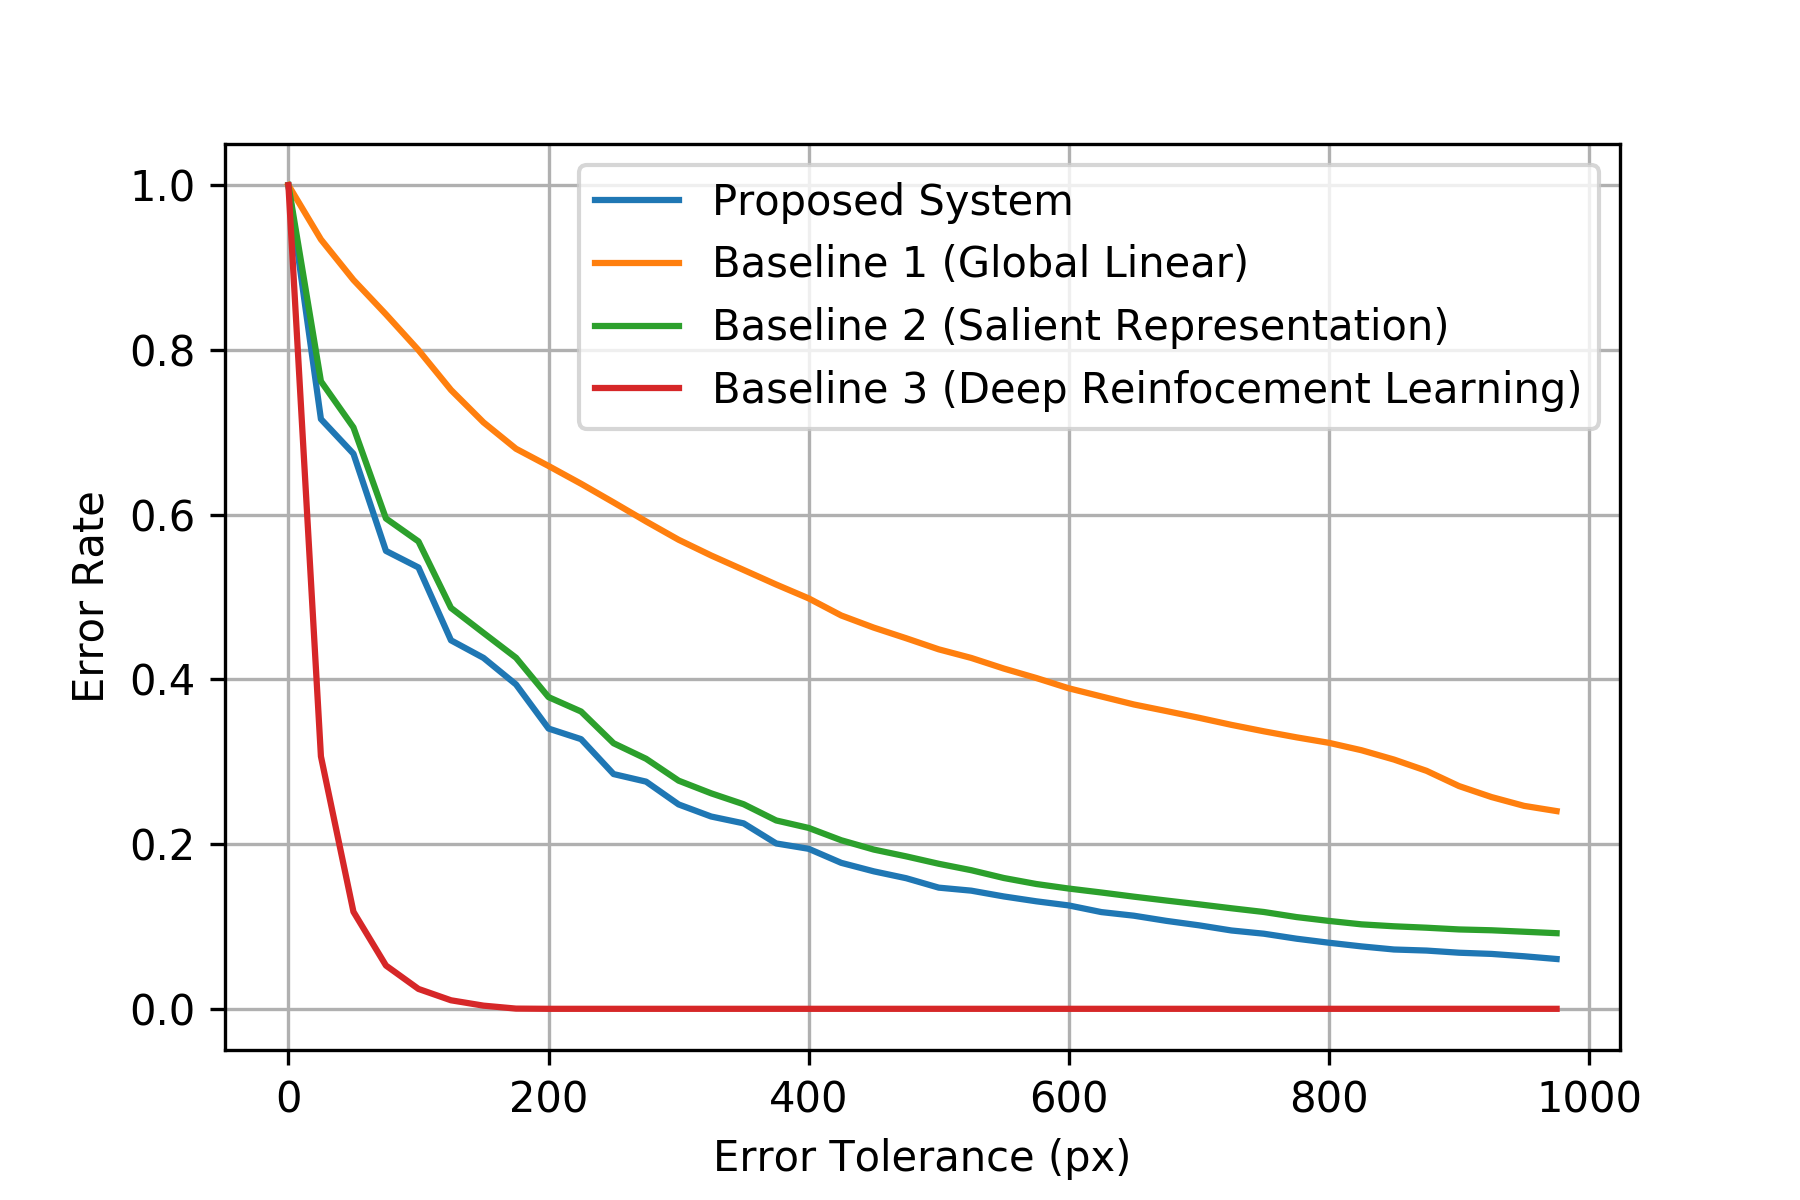
\includegraphics[scale=0.61]{images/final_result.png}
    \caption{Error Tolerance curve on 100 pieces from MSMD dataset}
    \label{fig:result}
\end{figure}
\begin{table}[]
    \centering
    \begin{tabular}{c|c|c}
        \textbf{System} & $\overline{|d_x|}$ & $std(|d_x|)$ \\\hline\hline
        Proposed System & 249.12 px & 367.62 px\\
        Baseline 1 & 623.34 px & 631.68 px\\
        Baseline 2 & 330.01 px & 540.36 px\\
        Baseline 3 \cite{dorfer} & 23.11 px & 25.52 px 
    \end{tabular}
    \caption{Mean and Standard Deviation of Absolute Error}
    \label{tab:result}
\end{table}

The first global linear baseline system performs the worst. This implies that the problem of sheet music following is not trivial. The third state-of-the-art baseline system based on deep reinforcement learning performs the best with very small errors. Compared with this baseline system, our system performed much worse. This may suggest that it is possible to adopt techniques done in the deep reinforcement learning baseline \cite{dorfer} to improve our system’s performance. Comparing with the second baseline system that uses audio salience representation, we observe a tiny improvement. This indicates that the log-frequency spectrogram is more suitable representation for doing the task of sheet music following.

Investigating the performance gap between our proposed system and the baseline system with deep reinforcement learning, we found that long pieces that have more than 8 sheet music strips tend to significantly worsen our system's performance. However, on shorter pieces, we observed that our system is competitive with the deep reinforcement learning baseline. This implies that the major contribution of prediction errors come from extreme re-scaling factor for converting a log-frequency spectrogram into its bootleg representation.

\section{CONCLUSIONS}
In this paper, we have demonstrated a simple DTW algorithm for sheet music following task by using a feature representation resembling coarse estimation of sheet music containing only noteheads called a soft bootleg score. The bootleg score contains only rectangular floating notehead blobs. We evaluate the proposed system on a dataset of 100 synthesized piano scores. Our results indicate that the proposed approach work decently on piano music. However, the state-of-the-art system based on deep reinforcement learning still outperforms our system by a significant margin. As a trade-off, this deep reinforcement learning system requires a significant amount of training, and the training is done in a simulated environment. We note that our proposed system does not involve any training and can be adapted very easily to handle other kind of music, such as other instruments or other types of music (e.g. string quartet).

Since our proposed method can perform a score following task based on a simple bootleg synthesis from log-frequency spectrogram, we believe that incorporating the state-of-the-art work on automatic piano transcription from audio signal would be a great comparison and may lead to a very interesting result. Furthermore, the future work should also include eliminating irrelevant symbolic representations that are not noteheads in the synthesized bootleg score by performing noteheads detection using convolutional neural networks.


\bibliographystyle{IEEEtran}
\addtolength{\textheight}{-12cm}   % This command serves to balance the column lengths
                                  % on the last page of the document manually. It shortens
                                  % the textheight of the last page by a suitable amount.
                                  % This command does not take effect until the next page
                                  % so it should come on the page before the last. Make
                                  % sure that you do not shorten the textheight too much.

%%%%%%%%%%%%%%%%%%%%%%%%%%%%%%%%%%%%%%%%%%%%%%%%%%%%%%%%%%%%%%%%%%%%%%%%%%%%%%%%



%%%%%%%%%%%%%%%%%%%%%%%%%%%%%%%%%%%%%%%%%%%%%%%%%%%%%%%%%%%%%%%%%%%%%%%%%%%%%%%%



%%%%%%%%%%%%%%%%%%%%%%%%%%%%%%%%%%%%%%%%%%%%%%%%%%%%%%%%%%%%%%%%%%%%%%%%%%%%%%%%
% \section*{APPENDIX}

% Appendixes should appear before the acknowledgment.

% \section*{ACKNOWLEDGMENT}

% The preferred spelling of the word �acknowledgment� in America is without an �e� after the �g�. Avoid the stilted expression, �One of us (R. B. G.) thanks . . .�  Instead, try �R. B. G. thanks�. Put sponsor acknowledgments in the unnumbered footnote on the first page.



%%%%%%%%%%%%%%%%%%%%%%%%%%%%%%%%%%%%%%%%%%%%%%%%%%%%%%%%%%%%%%%%%%%%%%%%%%%%%%%%

\begin{thebibliography}{99}
\bibitem{dorfer} 
Matthias Dorfer, Florian Henkel, and Gerhard Widmer.
``Learning to Listen, Read, and Follow: Score Following as a Reinforcement Learning Game'', 
\textit{in Proceedings of the 19th International Society for Music Information Retrieval Conference (ISMIR)}, 2018, pp. 784-791.

\bibitem{dorfer2} 
Matthias Dorfer, Andreas Arzt, and Gerhard Widmer.
``Towards score following in sheet music images'', 
\textit{in Proceedings of the 17th International Society for Music Information Retrieval Conference (ISMIR)}, New York City, United States, 2016, pp. 789-795.

\bibitem{dorfer3}
Matthias Dorfer, Andreas Arzt, and Gerhard Widmer.
``Learning audio-sheet music correspondences for score identification  and  offline alignment'', 
\textit{in Proceedings of the 18th  International Society for Music Information Retrieval Conference (ISMIR)}, Suzhou, China, 2017, pp. 115-122.

\bibitem{dtw1} 
Roger B. Danenberg and Ning Hu.
``Polyphonic audio matching for score following and intelligent audio editors,''
\textit{in Proceedings of the International Computer Music Conference (ICMC)}, San Francisco, USA, 2003, pp. 27-34.
 
\bibitem{dtw2} 
Sebastian Ewert, Meinard M\"uller, and Peter Grosche.
``High resolution audio synchronization using chroma onset features,''
\textit{in Proceedings of IEEE Internatinoal Conference on Acoustics, Speech, and Signal Processing (ICASSP)}, Taipei, Taiwan, Apr. 2009, pp. 1869-1872.

\bibitem{page_turning}
Andreas Arzt, Gerhard Widmer, and Simon Dixon.
``Automatic page turning for musicians via real-time machine listening,''
\textit{in Proceedings of the 18th European Conference on Artificial Intelligence (ECAI)}, Patras, Greece, 2008, pp. 241-245.

\bibitem{accompaniment1}
Arshia Cont. 
``A coupled duration-focused architecture for realtime music to score alignment,''
\textit{IEEE Transactions on Pattern Analysis and Machine Intelligence}, 32(6):837-846, 2009.

\bibitem{accompaniment2}
Christopher Raphael.  
``Music  Plus  One  and  machine learning,'' 
\textit{in Proceedings of the International Conference on Machine Learning (ICML)}, 2010.

\bibitem{live1}
Andreas Arzt, Harald  Frostel, Thassilo Gadermaier, Martin Gasser, Maarten Grachten, and Gerhard Widmer.  
``Artificial intelligence in the concertgebouw,''  
\textit{in Proceedings of the Twenty-Fourth International Joint Conference on Artificial Intelligence (IJCAI)}, Buenos Aires, Argentina, 2015, pp. 2424-2430. 

\bibitem{live2}
Matthew Prockup, David Grunberg, Alex Hrybyk, and Youngmoo E. Kim. 
``Orchestral performance companion:  Using real-time audio to score alignment,''
\textit{IEEE Multimedia}, 20(2):52-60, 2013

\bibitem{omr_based1}
Frank Kurth, Meinard M\"{u}ller, Christian Fremerey, Yoon-Ha Chang, and Michael Clausen.
``Automated synchronization of scanned sheet music with audio recordings,'' 
\textit{in Proceedings of the International Conference on Music Information Retrieval (ISMIR)}, Vienna, Austria, Sept. 2007, pp. 261-266.

\bibitem{omr_based2}
Verena Thomas, Christian Fremerey, Meinard M\"{u}ller, and Michael Clausen, ``Linking sheet music and audio---challenges and new approaches,'' 
\textit{in Multimodal Music Processing},
Meinard M\"{u}ller, Masataka Goto, and Markus Schedl, Eds., vol. 3 of Dagstuhl Follow-Ups, pp. 1-22. Schloss Dagstuhl-Leibniz-Zentrum f\"{u}r Informatik, Dagstuhl, Germany, 2012

\bibitem{msmd}
Matthias Dorfer, Jan Haji\v{c} jr., Andreas Arzt, Harald Frostel, and Gerhard Widmer. 
``Learning Audio-Sheet Music Correspondences for Cross-Modal Retrieval and Piece Identification,'' 
\textit{Transactions of the International Society for Music Information Retrieval}, issue 1, 2018.

\bibitem{madmom}
Sebastian B{\"o}ck, Filip Korzeniowski, Jan Schl{\"u}ter, Florian Krebs, and Gerhard Widmer.
``madmom: a new Python Audio and Music Signal Processing Library,''
\textit{in Proceedings of the 24th ACM International Conference on Multimedia}, Amsterdam, The Netherlands, Oct. 2016, pp. 1174-1178.

\bibitem{onset}
Juan Pablo Bello, Laurent Daudet, Samer Abdallah, Chris Duxbury, Mike Davies, and Mark B. Sandler.
``A tutorial on onset detection in music signals,''
\textit{in IEEE Transactions on Speech and Audio Processing}. 13(5), Part 2,  September, 2005, pp. 1035-1047.

\end{thebibliography}




\end{document}
